\newpage
\section{Testiranje i rezultati}
\subsection{Metodologija testiranja}
Način testiranja je ugraditi projekt u automobil te testirati njegov rad tijekom vožnje. Očekivano ponašanje je ispravan prikaz brzine automobila, obrtaja te trenutne brzine mjenjača na ekranu. Ispravnost prikaza se određuje usporedbom prikazaninh vrijednosti s pokaznicima brzine, obrtaja i trenutne brzine koji se tvornički nalaze u automobilu. Dozvoljeno je malo odstupanje zbog nepreciznosti pokazivača koji se nalaze već par desetljeća u automobilu. Pored Navedenih indikatora tu su još i indikatori za razinu spremnika, temperaturu motora automobila, ukupan broj prijeđenih kilometara te projsečnu potrošnju na 100 kilometara čija točnost se procjenjuje na isti način koji je prethodno naveden. Nadalje, testira se i funkcionalnost multimedije na način da se prikazuje izbornik za radiostanice kao i mogućnost reprodukcije multimedijskog sadržaja iz neke vanjske memorije npr. USB uređaj za pohranu podataka.

\subsection{Rezultati testiranja}
Prvo je testiran prikaz telemetrije automobila čiji prikaz je vidljiv na slici \ref{fig:car_telemetry}. Uzastopnim vožnjama i prometnim kamerama je utvrđeno kako se na ekranu prikazuje točna vrijednost brzine automobila i obrtaja motora. Kako se brzina mjenjača računa na osnovu obrtaja i brzine kretanja automobila, to je veličina koja bi bila podložna greškama u izračunama međutim u praksi se pokazalo kao vjerodostojan izračun bez krivih indikacija. Indikatori razine spremnika goriva, temperaturu motora automobila te prosječna potrošnja se podudaraju s vrijednostima prikazanih na glavnoj tabli čime zaključujemo kako sva komunikacija ispravno radi.
\begin{figure}[H]
    \centering
    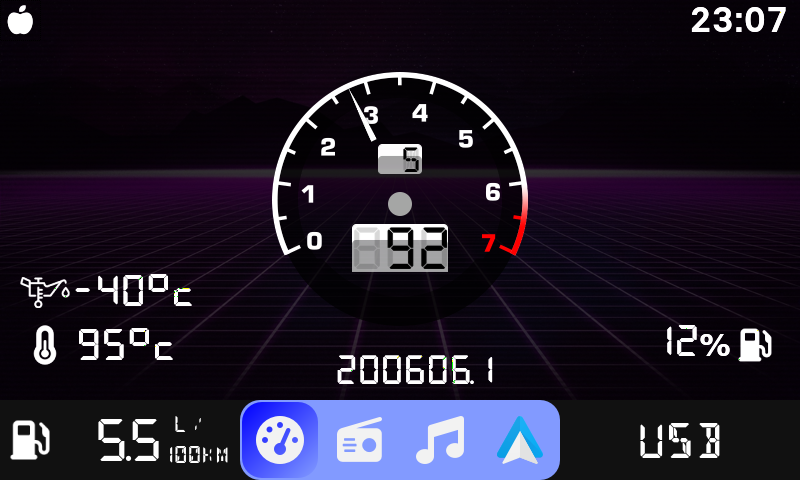
\includegraphics[width=0.75\textwidth]{images/1-rpm.png}
    \caption{Prikaz ekrana tijekom testiranja - Telemetrija automobila}
    \label{fig:car_telemetry}
\end{figure}

Na slici \ref{fig:car_multimedia_external_storage} je prikazan test učitavanja multimedijskog sadržaja sa vanjskog uređaja za pohranu podataka. Kako je sadržaj bez ikakvih problema učitan te reproduciran, zaključuje se kako i taj dio sustava radi kao što je predviđeno.

\begin{figure}[H]
    \centering
    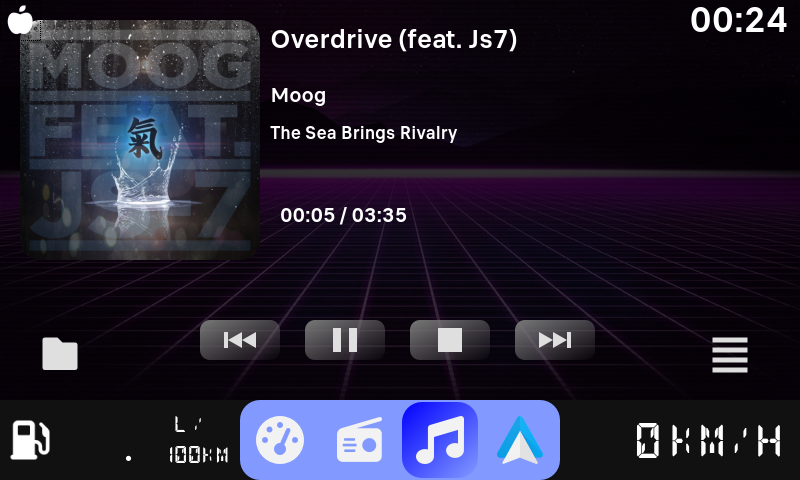
\includegraphics[width=0.75\textwidth]{images/2-musicplayer.png}
    \caption{Prikaz ekrana tijekom testiranja - Multimedija - Uređaj za pohranu podataka}
    \label{fig:car_multimedia_external_storage}
\end{figure}

Na slikama \ref{fig:car_multimedia_radio} i \ref{fig:radio} je prikazan test prikaza aktivne radio stanice (ukoliko je radio upaljen) iz kojih se može vidjeti kako i ta funkcionalnost ima predviđeno ponašanje.

\begin{figure}[H]
    \centering
    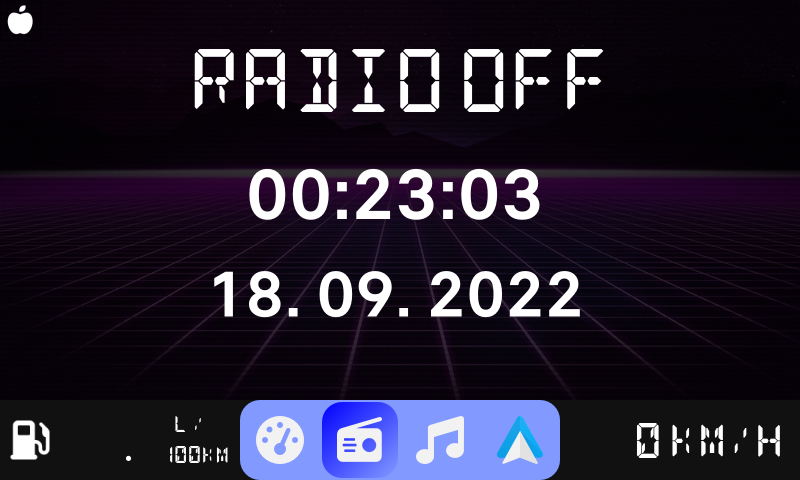
\includegraphics[width=0.75\textwidth]{images/3-radiooff.png}
    \caption{Prikaz ekrana tijekom testiranja - Multimedija - Radio}
    \label{fig:car_multimedia_radio}
\end{figure}

\begin{figure}[H]
    \begin{center}
        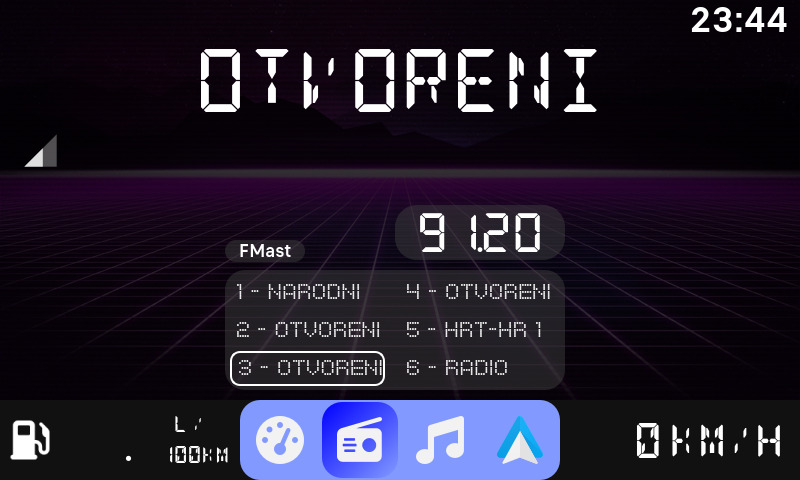
\includegraphics[width=0.75\textwidth]{images/radio.jpeg}
        \caption{Infotainment sustav smješten u autu}
        \label{fig:radio}
    \end{center}
\end{figure}